% IEEE standard conference template; to be used with:
%   spconf.sty  - LaTeX style file, and
%   IEEEbib.bst - IEEE bibliography style file.
% --------------------------------------------------------------------------

\documentclass[letterpaper]{article}
\usepackage{spconf,amsmath,amssymb,graphicx}
\usepackage{graphicx}
\usepackage{tabularx}
\usepackage[export]{adjustbox}
\usepackage{float}
\usepackage{array}
\usepackage{amsmath}
\usepackage{algorithm}
\usepackage[noend]{algpseudocode}

%\usepackage{caption}
\usepackage{subcaption}


% Example definitions.
% --------------------
% nice symbols for real and complex numbers
\newcommand{\R}[0]{\mathbb{R}}
\newcommand{\C}[0]{\mathbb{C}}

% bold paragraph titles
\newcommand{\mypar}[1]{{\bf #1.}}

% Title.
% ------
\title{Predictions of urban qualities in the city of Zurich}
%
% Single address.
% ---------------
\name{Jakub Lichman, Philippe Schlattner, Florian Koch}
\address{Department of Computer Science\\ ETH Zurich\\Zurich, Switzerland}

% For example:
% ------------
%\address{School\\
%		 Department\\
%		 Address}
%
% Two addresses (uncomment and modify for two-address case).
% ----------------------------------------------------------
%\twoauthors
%  {A. Author-one, B. Author-two\sthanks{Thanks to XYZ agency for funding.}}
%		 {School A-B\\
%		 Department A-B\\
%		 Address A-B}
%  {C. Author-three, D. Author-four\sthanks{The fourth author performed the work
%		 while at ...}}
%		 {School C-D\\
%		 Department C-D\\
%		 Address C-D}
%

\begin{document}
%\ninept
%
\maketitle
%

\begin{abstract}
We should do as the last one.
\end{abstract}

\section{Introduction}\label{sec:intro}
Huge predicted increase in number of world urban area residents from 54 to 66 percent in 2050 brings many challenges 
which every successful city has to overcome. Cities of the future has to ensure contiguous improvements of their 
services despite growing population. Since it is infeasible for a city to excellent in all services, 
authorities have to reach compliance about the subset of prioritized ones. For instance, this year's Mercer's Quality of Living index 
%[https://mobilityexchange.mercer.com/Insights/quality-of-living-rankings] 
takes into account economic and political environment, infrastructure, public transport, health, recreation and housing, 
to decide which cities are most desirable. Based on these factors, the list of most livable cities was constructed. 
However these types of rankings usually generalize the whole city and take average of the all districts which can 
over or underrate them. In our paper we tried to distinguish urban qualities within a city, concretely in the city of Zürich. 
Its public data availability enabled us to make interesting predictions about urban qualities of individual city districts 
which we lately verified by examining selected places in person. 
%[https://www.telegraph.co.uk/travel/galleries/The-worlds-most-liveable-cities/]

\indent Our experiment tries to exploit data that are publicly available for the city of Zurüich as well as data that we tried to obtain by ourselves. 
The goal was to create a map of the city with multiple layers where each layer will represent one factor of urban quality. By summing all factors and 
visualizing them we can obtain an interactive map which visualizes livability of each part of the city. Later we evaluated selected areas with smart
Agora platform which enabled us to collect data for validation by walking of these areas.

\section{Background}\label{sec:background}
TODO: Write about smart cities etc.

\section{Related Work}
TODO: Cite few similar papers

\section{Data}\label{sec:data}
To begin with, we evaluated data downloaded from the open data initiative of the city of Zurich \cite{ZurichOD}. 
Furthermore, we used maps from the Geographic Information System of the canton of Zurich GISZH \cite{GISZH} to get 
an idea of potentially interesting areas.
These two sources were used, since we believed that data published by institutions of the government is in general 
more reliable than that published by individuals. In addition, the data is considered to be of better quality and 
cover more of the area. This initial trust has been partially disappointed by finding quite a few data sets with only few points.
As we wanted to predict the best living areas within Zurich, we also need data that covers more or less the complete area of Zurich
in order to avoid bias towards certain regions, which are better covered by the data sources. Therefore, we ommited data sets 
with subjectively too few entries, which we initially wanted to use due to their potential. These omitted data sets include 
the one on air quality, flat prices and traffic counts.
The data we finally used and analysed is composed of data for public street illumination, pedestrian zones, sighing points, 
zones where driving is prohibited as well as restaurants. These are all sets where the available data is spread across 
a large part of Zurich and that we figured might be indicative for how much we as students would appreciate living there. 
This is a highly subjective measure that took us some time to agree amongst ourselves.
The analysis of the data is described in Sec. \ref{sec:predictions}. In addition we inferred the amount of greenery from satellite 
images as outlined in Sec. \ref{sec:greenery} to evaluate how urban the areas are. Finally we tried to evaluate the predictions 
by having people walk some of the areas and gather their impression by utilising Smart Agora. The details of the last bit 
are outlined in Sec. \ref{sec:exp}.

\section{Measure of Attractiveness}\label{sec:attractiveness}
As we are all students at ETH Zurich, we wanted to map the attractiveness to live in a certain area from the point of view students have. 
Therefore, access to public transport is important, however walking for up to 15 minutes does not bother us that much. Hence, we did not 
include stops of public transportation in our analysis, since they are well anough distributed that we found a stop is in wlaking distance 
to each and every location within Zurich.
On the other hand we did not have access to detailed data on diverse measures. Accordingly we defined spheres of influence for all types 
of points we used for the analysis, that should represent how far we believe that item will influence how we perceive the area.
This also means that accessibility for example is not that relevant, compared to bars and restaurants. Another factor that is 
very important to us was the proximity to places we visit frequently. However, this is even more subjective and even in our 
small group of people we could not identify several points of interest, that are common to all of us except for study related locations.

\section{Greenery Detection}\label{sec:greenery}
\indent Greenery has always played crucial part in the construction of cities. The need for green spaces has been present since ancient times.
City parks are traditional place of recreation and relax for all kinds of people in their spare time. Current trends in architecture brought new ways of
connecting buildings and greenery such as roofs with green surfaces or terraces with tree pots. These trends are consequence of natural 
human inclination towards nature. Therefore we have decided to take greenery as a significant indicator of urban quality.

\indent In order to predict user preferences partially based on greenery, we needed to acquire data about it. There are two basic ways how to detect trees, 
parks or grass areas on a map. First approach relies on a snapshot of a satellite view \cite{smartCities}. It is simple to implement and yields accurate results. 
Detection of green areas is via pixels with RGB values that lie within specified intervals. The only crucial requirement in order to obtain precise detection 
is to find high quality satellite view of the selected area. 
Second approach is to detect greenery from Google Street View (GSV) \cite{googleView}. Xiaojiang Li et. al. detected greenery by examining street
pictures taken from GSV. With this method they were able to explore greenery inside the cities in great detail. Idea behind second method is in general
more accurate since it can detect trees shadowed by taller buildings or shelters. However, its precision highly depends on availability of street view and
algorithms, which are in our view still not accurate enough. That is the reason why we have decided to use the first method.

\indent We developed the python script which does greenery detection similarly to the first approach mentioned above. 
Firstly, we did the transformation of RBGA pixel format into HSV one where detection of color spectrum is more accurate.
However during searching for the right green space we encountered few issues. Detection of grasslands together 
with forests was infeasible within a single interval. While grasslands are pixels of a bright green, forests are 
the ones with a very dark one together with a dark grey in the locations where one tree shadows the other. 
Therefore we had to distinguish between them and thus do two separate detections. Combination of them then 
produced desired result. Detection of forests, grasslands and their combination can be seen in the Figure~\ref{fig:ZurichGreenery}

\begin{figure}
    \centering
    \begin{subfigure}{.22\textwidth}
        \centering
        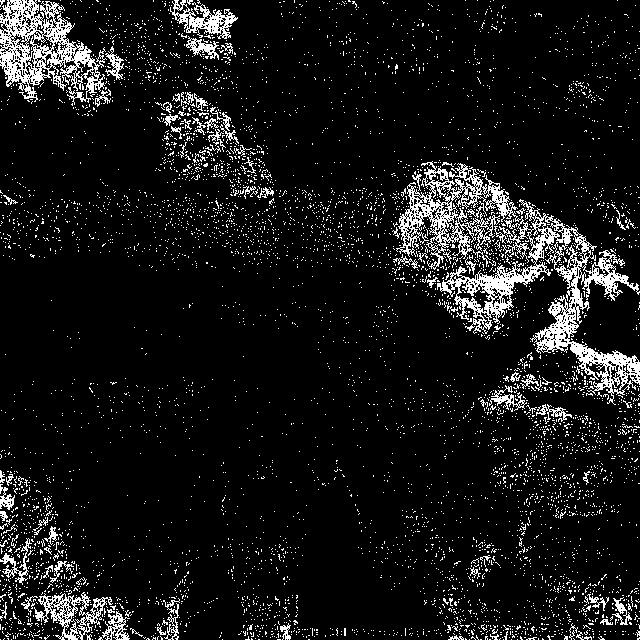
\includegraphics[width=.95\linewidth]{../images/greenery/forests.png}
        \caption[width=.2\textwidth]{Mask of the forests}
    \end{subfigure}%
    \begin{subfigure}{.22\textwidth}
        \centering
        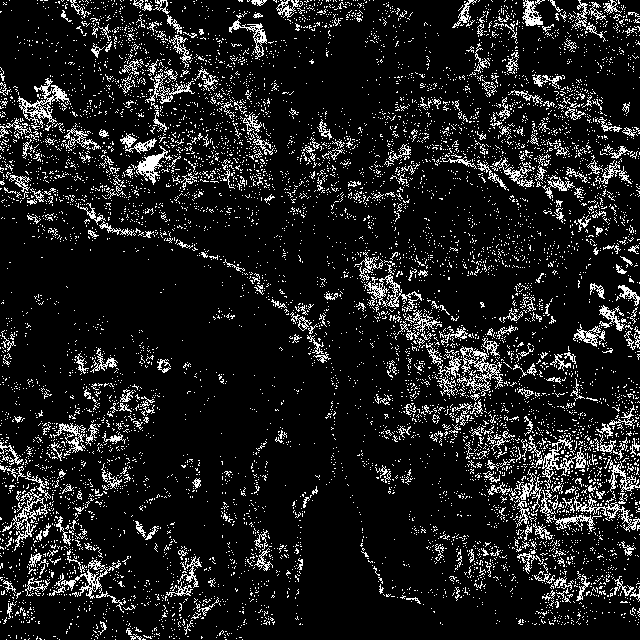
\includegraphics[width=.95\linewidth]{../images/greenery/green_areas.png}
        \caption[width=.2\textwidth]{Mask of the grasslands}
    \end{subfigure}

    \begin{subfigure}{.22\textwidth}
        \centering
        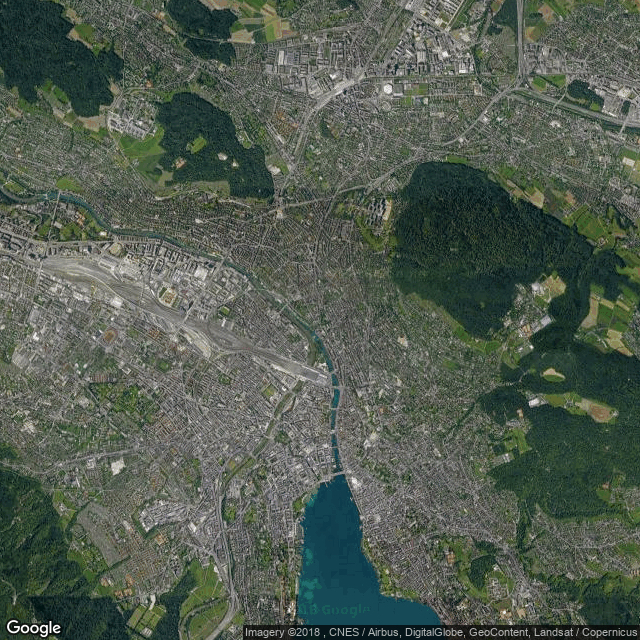
\includegraphics[width=.95\linewidth]{../images/greenery/Zurich.png}
        \caption[width=.2\textwidth]{Unmodified Zürich area}
    \end{subfigure}%
    \begin{subfigure}{.22\textwidth}
        \centering
        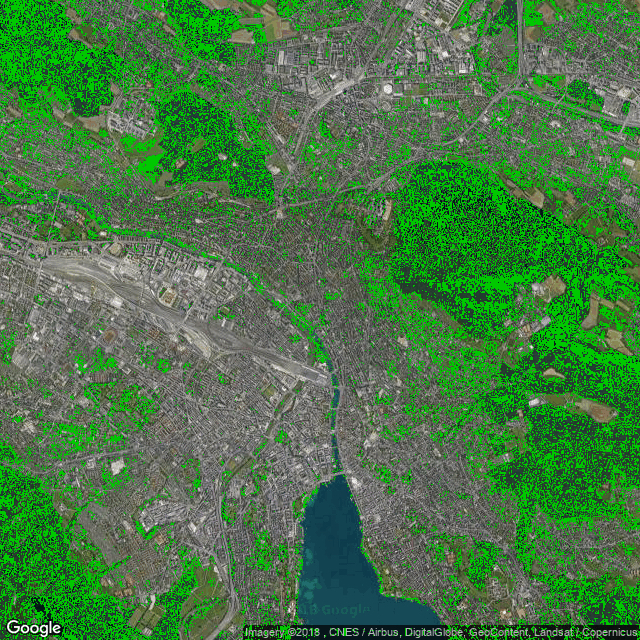
\includegraphics[width=.95\linewidth]{../images/greenery/Zurich_greenery.png}
        \caption[width=.2\textwidth]{Greenery in the Zürich area}
    \end{subfigure}
    \caption{Visualization of the greenery detection phases. In the original image we firstly detected forests then 
             grasslands and finally we combined them and overlay above the original image.}
    \label{fig:ZurichGreenery}
\end{figure}

Detected locations are marked with the RGB value (0, 200, 0) which is solid green. Furthermore our method computes intensity matrix which indicates influence
of the detected greenery on every place within the city of Zürich. Our approch firstly produces binary matrix $B$ of the image $P$ with greenery
locations $G$ such that 
\newline
\begin{align*}
B_{i,j} = \begin{cases} 1 & \text{if } P_{i,j} \in G\\
                         0 & \text{if } P_{i,j} \notin G  
\end{cases}
\end{align*}
\newline
In the second phase we perform "smoothing" which in every iteration visits every entry in the matrix and checks all neighbouring pixels, 
finds maximum of them and assigns its half to the current pixel. More formally:

\begin{algorithm}
    \caption{Smoothing}\label{smooth}
    \begin{algorithmic}[1]
    \Procedure{Smoothing}{iterations, B}
    \State $\textit{S} \gets \textit{B}$
    \State $\textit{i} \gets \textit{0}$
    \State $\textbf{while } \textit{i} < 0:$
    \State $\indent \textbf{forall } p \textbf{ in } S:$
    \State $\indent \indent p := max_{neighbours}(p) / 2$
    \State $\indent \textit{i} \gets \textit{i} + 1$
    \EndProcedure
    \end{algorithmic}
    \end{algorithm}
    
We can see the effect of Smoothing~\ref{smooth} on Matrix~\ref{eq:MatA} after 2 iterations
in Matrix~\ref{eq:MatB}. Remaining $0$ entries would be replaces $0.125$ after third iteration.

\begin{equation}
\begin{pmatrix}
    0 & 0 & 0 & 0 & 0 \\
    0 & 0 & 0 & 0 & 0 \\
    0 & 0 & 0 & 0 & 0 \\
    0 & 0 & 0 & 1 & 0 \\
    0 & 0 & 0 & 0 & 0 \\
\end{pmatrix}
\label{eq:MatA}
\end{equation}
\begin{equation}
\begin{pmatrix}
    0 & 0 & 0 & 0 & 0 \\
    0 & 0.25 & 0.25 & 0.25 & 0.25 \\
    0 & 0.25 & 0.5 & 0.5 & 0.5 \\
    0 & 0.25 & 0.5 & 1 & 0.5 \\
    0 & 0.25 & 0.5 & 0.5 & 0.5 \\
\end{pmatrix}
\label{eq:MatB}
\end{equation}
Snapshot of selected location was taken from Google maps satellite view.

\section{Urban quality prediction}\label{sec:predictions}
TODO: This should be "core" chapter of our paper. Philippe here you can describe whole procedure of data visualization + correlation matrix etc.

\section{Predictions evaluation}\label{sec:exp}
For evaluating the predictions we derived in the previous section, we chose to let people rate that areas based on their visual impression after walking through the respective part of the city. For this we initially wanted to use Smart Agora, as it allows to pose the questions at various locations.

\begin{figure}[htb]
    \centering
    \includegraphics[width=\columnwidth]{../images/greenery/Zentrum_greenery.png}
    \caption{Greenery detection in the area of our path.}
    \label{fig:path_greenery}
\end{figure}

\begin{figure}[htb]
	\centering
	\includegraphics[width=\columnwidth]{../images/greenery/Zentrum_path.png}
	\caption{Locations of question points along the path}
	\label{fig:path_points}
\end{figure}

After setting up some test paths and questions for people to walk, we decided to abandon this approach as the usability for both experimenter and participant is at this stage not acceptable. Some of the improvements we deem neccessary are outlined in Sec. \ref{sec:discussion}.

\section{Discussion}\label{sec:discussion}
TODO: Discuss possible drawback and ways how to improve them + results and whether we are satisfied with our predictions.

\section{Conclusion}\label{sec:conclusion}
We should do as the last part together with abstract.


\bibliographystyle{IEEEbib}
\bibliography{report.bbl} %pick these locations + photos of walking and measured re-

\section{Appendix}

\end{document}
